% ----- THIS SECTION COPIED FROM AJP GUIDELINES sample doc

\documentclass[prb,preprint]{revtex4-1} 
%\documentclass[12pt]{article}

\usepackage{amsmath}
\usepackage{amsfonts} % needed for bold Greek, Fraktur, and blackboard bold
\usepackage{graphicx} % needed for figures 
\usepackage{multirow} % needed for table

% ----- end --- THIS SECTION COPIED FROM AJP GUIDELINES sample doc

\usepackage{tabu}
\graphicspath{ {images/} }

\begin{document}
\title{High-precision determination of accelerometer positions using a linear regression technique}



\begin{abstract}
A better way of determining positions is presented..
\end{abstract}

\maketitle
\section{Introduction}

Review previous work..

\section{Methods and Results}
We follow the same approach described in \cite{LarnderLarade}. The host device is placed on a horizontal surface which is then rotated at a known angular rate omega. The position of the device.. at a known position in a 2-D coordinate system whose origin coincides with the axis of rotation...

\subsection{Preliminary demonstrations}
The behaviour one would intuitively expect from operating a device that hosts an accelerometer is that acceleration values correspond to the dynamics occurring either at the geometrical center of the device or as an average over the entire surface of the device. This assumption can be quickly disproved by a simple preliminary experiment.
 
Fig.~\ref{fig:TwoPositions} shows two device positions for which the central-location assumption would result in a radial acceleration being measured along a single axis. In device position A, for example, if the true intra-device sensor position were anywhere along the central left-right axis, the resulting centripetal acceleration would be non-zero only along the (positive side of the) x-axis. For most host devices this will not be the case, and moreover the sign of the non-zero y-axis component will indicate whether the true position is above or below that central axis, as illustrated in Fig.~\ref{fig:NotAtCenter}. Similarly, when the device is in position B, the sign of the x-axis component tells the student whether the accelerometer position is to the left or to the right of the central up-down axis. From these simple observations, and without appealing to any mathematical equations, a student can already narrow down the location of the sensor to one of the four quadrants of the host device surface area. This activity sharpens the students' geometrical intuition and whets their appetite for a more methodical approach to finding the true sensor position.

\subsection{The linear regression method}

Consider the radial line that is perpendicular to a border of the frame shown in Fig. x. If the device is placed at a series of positions along that border, we will note the following behaviour of the acceleration components when in a condition of uniform circular motion:
i) the component perpendicular to the frame will remain constant ii) the component parallel to the border will change linearly, and, when the sensor reaches the radial line, it will change sign.
It is this change-of-sign behaviour that reveals the position of the sensor along that axis. A linear regression of all data points allows for an accurate determination.


%discussion


%acknowledgement hidden for review process
%This work was funded in part by a grant from the \textit{ Entente Canada-Qu\'{e}bec relative \`{a} l'enseignement % dans la langue de la minorit\'{e} et \`{a} l'enseignement des langues secondes.} 

\begin{thebibliography}{5}


\bibitem{LarnderLarade}
%1
C.I. Larnder and B. Larade,
''On the determination of accelerometer sensor positions in host devices,''
Am. J. Phys.
\textbf{87}, 130 (2019).


\end{thebibliography}

\begin{figure} [h]
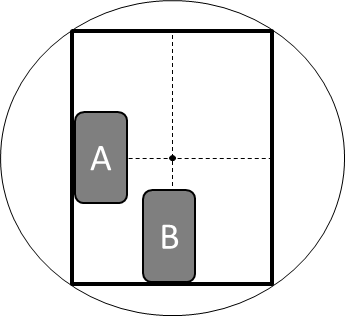
\includegraphics[width=14 cm]{TwoPositions}
\centering
\caption{Two device positions for disproving the centrality of accelerometer location }
\label{fig:TwoPositions}
\end{figure}


\begin{figure} [h]
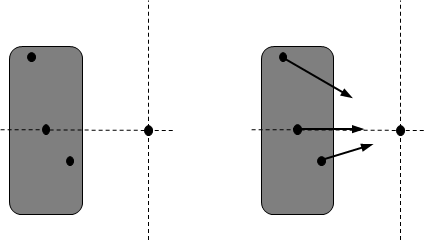
\includegraphics[width=14 cm]{NotAtCenter}
\centering
\caption{Three hypothetical intra-device locations ( left ) and their corresponding radially-oriented acceleration vectors (right ) for device location “A” of the previous figure }
\label{fig:NotAtCenter}
\end{figure}



\end{document}